\documentclass[border=5pt,convert={outfile=../_static/\jobname.svg}]{standalone}

\usepackage{tikz}

\begin{document}

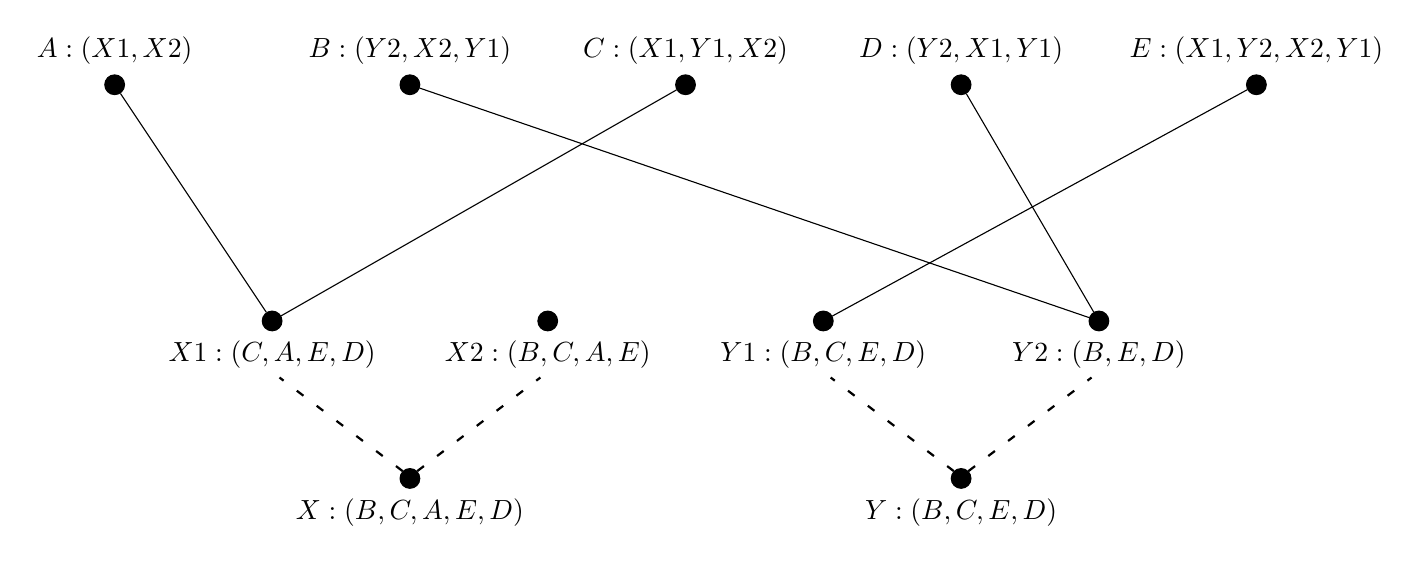
\begin{tikzpicture}[scale=0.5]

    % Students
    \node[draw, shape=circle, fill, inner sep=0, minimum size=0.25cm,
    label=above: {\(A: (X1, X2)\)}] (A) at (-4, 0) {};
    \node[draw, shape=circle, fill, inner sep=0, minimum size=0.25cm,
    label=above: {\(B: (Y2, X2, Y1)\)}] (B) at (3.5, 0) {};
    \node[draw, shape=circle, fill, inner sep=0, minimum size=0.25cm,
    label=above: {\(C: (X1, Y1, X2)\)}] (C) at (10.5, 0) {};
    \node[draw, shape=circle, fill, inner sep=0, minimum size=0.25cm,
    label=above: {\(D: (Y2, X1, Y1)\)}] (D) at (17.5, 0) {};
    \node[draw, shape=circle, fill, inner sep=0, minimum size=0.25cm,
    label=above: {\(E: (X1, Y2, X2, Y1)\)}] (E) at (25, 0) {};

    % Projects
    \node[draw, shape=circle, fill, inner sep=0, minimum size=0.25cm,
    label=below: {\(X1: (C, A, E, D)\)}] (X1) at (0, -6) {};
    \node[draw, shape=circle, fill, inner sep=0, minimum size=0.25cm,
    label=below: {\(X2: (B, C, A, E)\)}] (X2) at (7, -6) {};
    \node[draw, shape=circle, fill, inner sep=0, minimum size=0.25cm,
    label=below: {\(Y1: (B, C, E, D)\)}] (Y1) at (14, -6) {};
    \node[draw, shape=circle, fill, inner sep=0, minimum size=0.25cm,
    label=below: {\(Y2: (B, E, D)\)}] (Y2) at (21, -6) {};
 
    % Supervisors
    \node[draw, shape=circle, fill, inner sep=0, minimum size=0.25cm,
    label=below: {\(X: (B, C, A, E, D)\)}] (X) at (3.5, -10) {};
    \node[draw, shape=circle, fill, inner sep=0, minimum size=0.25cm,
    label=below: {\(Y: (B, C, E, D)\)}] (Y) at (17.5, -10) {};

    % Associations
    \draw[loosely dashed, thick]
    (X.north west) -- ([yshift=-1.25cm]X1.south east);
    \draw[loosely dashed, thick]
    (X.north east) -- ([yshift=-1.25cm]X2.south west);
    \draw[loosely dashed, thick]
    (Y.north west) -- ([yshift=-1.25cm]Y1.south east);
    \draw[loosely dashed, thick]
    (Y.north east) -- ([yshift=-1.25cm]Y2.south west);

    % Matches
    \draw (X1) -- (A);
    \draw (X1) -- (C);
    \draw (Y1) -- (E);
    \draw (Y2) -- (B);
    \draw (Y2) -- (D);


\end{tikzpicture}

\end{document}
